\section{Correlation function construction}
\label{sec:CorrelationFunctionConstruction}
\subsection{Relative momentum}
\label{sec:RelativeMomentum}

This analysis studies two-particle correlations as a function of the one-dimensional relative momentum $k^*$.
To be precise, for a pair of particles with four-momenta $p_1$ and $p_2$, $k^*$ is the momentum of one the particles in the pair's center of mass frame.
It is defined as
\begin{equation}
\label{eq:kstar}
k^*= \sqrt{-k^\mu k_\mu},
\end{equation}
where $k^\mu$ is half of the four-vector relative momentum
\begin{equation}
\label{eq:kmu}
k^\mu = \frac{p_1^\mu - p_2^\mu}{2} -\frac{(p_1 - p_2)\cdot P}{2P^2}P^\mu,
\end{equation}
$P$ is the four-vector momentum sum.

The literature is inconsistent when it comes to the notation for relative momentum.
In some cases, $k^*$ refers both to the invariant quantity and to the four-vector.
In this thesis, we will try to consistently use $k^*$ to designate the invariant quantity, and use $k^\mu$ when speaking of four-momenta.
In some papers, $q$ or $q_{\mathrm{inv}}$ is used to represent the relative momentum.
Though we won't use $q$ in this analysis, for reference
$q^\mu = 2k^\mu$, and $q_{\mathrm{inv}} = 2 k^*$.


\subsection{Construction}
\label{sec:CFconstruct}

The correlation function is constructed as
\begin{equation}
\label{eq:CFDefinition}
C(k^*) = \frac{A(k^*)}{B(k^*)},
\end{equation}
where $A(k^*)$ is the two-particle distribution of the given event and $B(k^*)$ is the distribution of a reference event.  
In practice, the signal event histogram $A(k^*)$ is constructed by binning the $k^*$ value of each pair of particles in a single event, and repeating this for each event.  
The reference or background histogram is constructed by binning $k^*$ for pairs of particles taken from different events.  
The correlation function therefore is the ratio of the two-particle phase-space with correlated effects coming from interactions (the numerator) to the two-particle phase-space without correlated effects (the denominator).
Because the denominator pairs are uncorrelated, their two-particle phase space is essentially a convolution of two single-particle phase spaces.
Of course, the numerator pairs are also affected by the single-particle phase spaces.
We assume that the physics of the numerator pairs can be factorized to separate out the correlated physics effects and the single-particle phase space effects.
Thus, dividing by the background pair distribution leaves us with just the correlated physics effects, i.e.\ the correlation function. See Section \ref{sec:KooninPratt} for more details.

In order for the phase-space effects to divide out, it is of course necessary for the mixed events to resemble the true events.
For example, a mixed event where half the particles come from a central collision and half the particles come from a very peripheral collision would have a very different two-particle phase space than a central collision would.
Care is therefore taken to ensure that pairs are mixed from events with similar characteristics. 
Mixed events are required to have approximately the same centrality (bin width of 5\%) and primary vertex z-position (2 cm bin width).  
There are approximately five mixed events for each real event.  
When constructing pairs of V0s from the same event, the V0s are not allowed to share a daughter with the same track ID. 
The correlation functions are normalized to unity in the $ 0.3 < k^* < 0.5$ GeV/c range.

\subsection{Pair cuts}
\label{sec:PairWiseCuts}

Femtoscopic studies look at the relative momentum of particles, and often the most interesting physics lies at very low relative momentum (around 0.1 GeV/c and lower).  
As a result, two-track reconstruction effects such as track splitting and track merging, both of which occur for tracks with similar momenta and trajectories, can have a large effect on the measured results.  
Track splitting means that the track left by a single charged particle is reconstructed as two separate tracks. 
A track splitting-like effect can also occur from cutting out tracks with too many shared TPC clusters.
Track merging occurs when the tracks of two separate particles are reconstructed as a single track.  
For V0s, splitting/merging occurs on the level of the daughter tracks, and it affects the reconstruction of the parent V0s.
However, one must be somewhat cautious here, since there can be physics effects that lead to a suppression or enhancement of tracks that are close together.
In particular, small track separation correlates somewhat with small relative momentum, so effects that suppress (enhance) low-$k^*$ pairs may also lead to some suppression (enhancement) of low-average separation pairs.  

In this analysis, two-track reconstruction effects are combated via a cut on the average separation of daughter tracks from different $\Lambda/\bar{\Lambda}$.  
The average separation distance of two daughter tracks are computed at nine different radii of the TPC.  
The track positions are measured via AliExternalTrackParam::GetXYZatR() at the following radii: 85, 105, 125, 145, 165, 185, 205, 225, and 245 cm.  
Pairs of daugther tracks are made from one daughter from the first V0 and one daughter from the second V0. Pairs are made for all daughter combinations, and each type of pair is tracked separately.
For each pair of daughter tracks, their separation is computed at each of those radii, and their average separation is taken as the mean value. If a track does not have a value at a particular radius (e.g.\ a low $p_T$ track with a small radius of curvature), that position is excluded from the calculation of the mean.
Same- and mixed-event pairs are binned according to this separation distance.  
To obtain an estimate of the merging/splitting effects both distributions are then scaled by the number of pairs at high average separation distance (10+ cm), and a correlation function (same event pairs/ mixed event pairs) is created. 

To ensure that average separation distributions of mixed-event pairs are comparable to the same-event distributions, it is necessary to perform a shifting of the primary vertex for mixed events.  
Doing so allows the track separations to be calculated as though both events had the same primary vertex.  
Without this correction, the mixed-event distributions are biased by differences in the primary vertex location.  
One could imagine an extreme example of this if one used a 20 cm wide z-vertex bin.  
In that case, tracks from different events could be shifted relative to each other by as much as 20 cm. 

The average separation correlation functions for various V0 daughter combinations are available in Figure \ref{fig:AverageSeparationAllPairs}.  
We see that all like-sign pair combinations, as well as proton-antiproton, show a dip at low average separation.  
This dip tells us that there is a depletion of tracks that are close together. 
This depletion may come from track merging or from effects similar to track merging, such as the rejection of tracks that have too many shared TPC clusters.
For these pairs of tracks, we implement cuts at average separation value where the correlation function looks to reach unity.
These cuts are applied uniformly to same-event and mixed-event pairs.
pp and $\bar{\mathrm{p}}\bar{\mathrm{p}}$ pairs are cut if their separation lies below 12 cm, while $\pi^-\pi^-$, $\pi+\pi^+$, p$\pi^+$, $\bar{\mathrm{p}}\pi^-$ and p$\bar{\mathrm{p}}$ are cut below 10 cm.

For the other opposite-sign pairs, the splitting/merging picture is less clear, in great part due to the low statistics at low average separation.
First and foremost, this tells us that there is a very low phase space for finding oppositely charged particles. 
That should not be a surprise, as the ambient magnetic field accelerates them in opposite directions.
As it is not clear whether there exists splitting or merging from these pairs, a conservatively large average separation cut has been implemented. p$\pi^-$ and $\bar{\mathrm{p}}\pi^+$ are cut at 15 cm, and $\pi^-\pi^+$ are cut at 25 cm.

One alternative/complement to using an average separation cut would be to enforce a relative decay length cut, where V0s are not paired with each other if their difference between their lab frame decay length values is less than some cut value (e.g.\ a few cm).  
One advantage of this cut is that the decay lengths of the various particles should be independent of physics effects - i.e. independent of any quantum interference or final state interaction that might occur between the particles.  
Meanwhile, the decay length cut may minimize daughter splitting effects, as well as some merging of low- and mid-$p_{\mathrm{T}}$ daughters.  
High-$p_{\mathrm{T}}$ daughters may still be affected by merging, since higher-$p_{\mathrm{T}}$ particles have straighter trajectories in the TPC.  
A study of relative decay length has not been performed here, but it may prove useful to combat splitting/merging effects in future V0 analyses.

\begin{figure}[hbt]
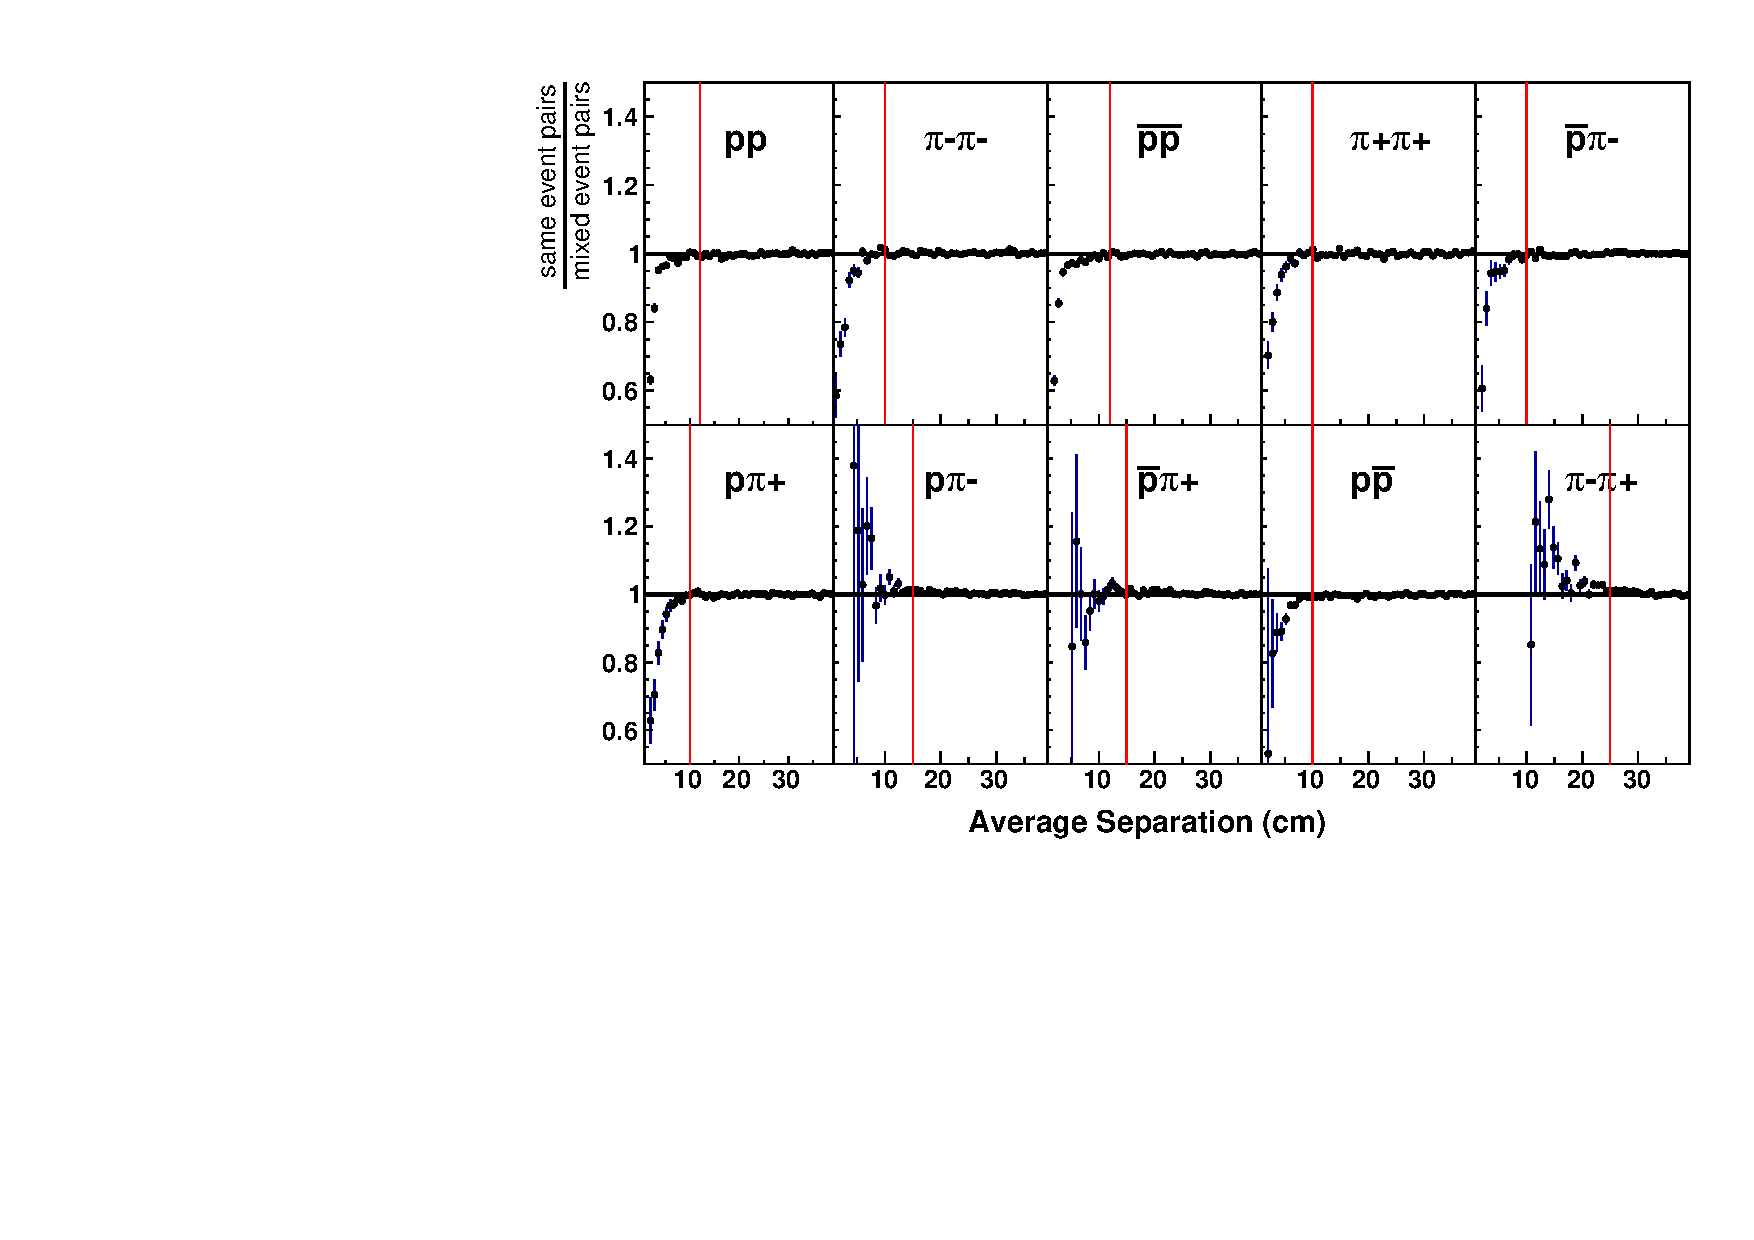
\includegraphics[width=36pc]{Figures/Cuts/2016-9-4-AllAvgSepCFs.pdf}
\caption[Average separation of V0 daughters]{
Correlation functions of average TPC track separation for pairs of daughters from different V0s. A correlation function is shown for each type of daughter combination. The positions of tracks are computed throughout the TPC, and an average separation value is calculated from those positions. This process is done for same- and mixed-event pairs. The correlation function reveals merging-like effects for all same-sign pairs and also for p$\bar{\mathrm{p}}$. To remove splitting/merging effects, V0 pairs are cut if  their daughters' average separation is below the indicated red line. Conservatively large cuts have been implemented for oppositely-charged pairs.}
\label{fig:AverageSeparationAllPairs}
\end{figure}

\subsection{Momentum resolution correction}
\label{sec:MomentumResCorrectionCF}

There is an inherent resolution to V0 momenta that depends on the resolution of the reconstructed daughter tracks.  
Because of this limit of precision, there is also an associated resolution to the relative momentum of two V0s.
This causes the reconstructed relative momentum of the pair to differ from the true momentum of the pair, and it therefore introduces subtle changes to the measured correlation functions which must be accounted for.

Tradionally, the momentum resolution correction is performed on the experimental data to unsmear it into a form that should resemble the theoretical predictions (i.e.\ fits). 
In this analysis we have instead chosen to smear the fits to conform to the experimental data. 
The experimental correlation functions therefore remain uncorrected. 
As our corrections are employed at the time of fitting, we'll discuss the full methodology in section \ref{sec:MomResCorrectFit}.